% Do not forget to include Introduction
%---------------------------------------------------------------
% \chapter{Introduction}
% uncomment the following line to create an unnumbered chapter
\chapter*{Úvod}
\addcontentsline{toc}{chapter}{Úvod}
\markboth{Úvod}{Úvod}
%---------------------------------------------------------------
\setcounter{page}{1}

% The following environment can be used as a mini-introduction for a chapter. Use that any way it pleases you (or comment it out). It can contain, for instance, a summary of the chapter. Or, there can be a quotation.
\begin{chapterabstract}
	\lipsum[1]
\end{chapterabstract}



%---------------------------------------------------------------
\chapter{Binární halda}
%---------------------------------------------------------------

\begin{definition}[Uložení haldy v poli]
...
\end{definition}


%---------------------------------------------------------------
\chapter{Implementace důkazu binární haldy}
%---------------------------------------------------------------

Tvar haldy umožňuje haldu efektivně uložit do lineárního pole a jednotlivé vrcholy očíslovat indexy pole. Tato ověřená implementace používá haldu s kořene na indexu $0$. Haldu uloženou v poli lze procházet pomocí těchto pravidel:

\begin{enumerate}
	\item[] $\Parent(i) = (i - 1) / 2$
	\item[] $\LeftChild(i) = 2i + 1$
	\item[] $\RightChild(i) = 2i + 2$
\end{enumerate}

Haldové uspořádání popisuje ACSL predikát \ref{acsl:ValidHeap}.

\begin{listing}[H]
	\caption{ACSL predikát validní haldy}
	\label{acsl:ValidHeap}
	\begin{minted}{c}
/*@
  predicate ValidHeap(Heap heap) =
    \forall integer ancestor, descendant;
      0 <= ancestor < descendant < HeapElementsCount(heap)
      && IsParent(ancestor, descendant) ==>
        HasHeapProperty(heap, ancestor, descendant);
*/
	\end{minted}
\end{listing}

Důkazy korektnosti byly provedeny v prostředí Frama-C 24.0 (Chromium) za použití externích dokazovacích nástrojů Alt-Ergo 2.2.0 a CVC4 1.7.

Výsledná implementace binární minimové haldy obsahuje 488 cílů pro důkaz korektnosti, splňuje korektní chování při použití RTE anotací a neobsahuje kontradikci ve vstupních podmínkách a nedosažitelný kód. RTE anotace se generují až při spuštění kontroly korektnosti pomocí přepínače "-rte". Kontradikce vstupních podmínek může způsobit úspěšné dokázání funkce, která ale nikdy nepůjde spustit, jelikož nelze splnit dané vstupní podmínky. Tuto kontrolu provádí "Smoke tests", které se spouštějí přepínačem "-wp-smoke-tests".

Kompletní důkaz celé knihovny binární minimové haldy lze spustit příkazem zobrazeným ve výpisu kódu \ref{shell:run-frama-c-proofs}.

\begin{listing}[H]
	\caption{Příkaz pro spuštění kompletního důkazu knihovny binární minimové haldy}
	\label{shell:run-frama-c-proofs}
	\begin{minted}{sh}
frama-c -rte -wp -wp-prover alt-ergo,cvc4 \
  -wp-par 8 -wp-cache none -wp-timeout 30 \
  -wp-smoke-tests -wp-smoke-timeout 30 \
  src/min_heap.c
	\end{minted}
\end{listing}

Výpis kódu \ref{shell:run-frama-c-proofs-output} zobrazuje výsledek provedení kopletního formálního důkazu knihovny binární minimové haldy. Tento výpis zobrazuje seznam všech funkcí, ve kterých byly vygenerované RTE automatické anotace společně s počtem nalezených cílů, které mají být v průběhu provádění důkazu korektnosti splněny. Knihovna splňuje všechny zapsané a vygenerované cíle. Výsledkem je tedy korektní implementace binární minimové haldy.

\begin{listing}[H]
	\caption{Výstup spuštění kompletního důkazu knihovny binární minimové haldy}
	\label{shell:run-frama-c-proofs-output}
	\begin{minted}{text}
...
[rte] annotating function HeapBubbleDown
[rte] annotating function HeapBubbleUp
[rte] annotating function HeapBuild
[rte] annotating function HeapChange
[rte] annotating function HeapDecrease
[rte] annotating function HeapElementValue
[rte] annotating function HeapExternalNodeCount
[rte] annotating function HeapExtractMin
[rte] annotating function HeapFindMin
[rte] annotating function HeapHasBothChildren
[rte] annotating function HeapHasChild
[rte] annotating function HeapHasLeftChild
[rte] annotating function HeapHasParent
[rte] annotating function HeapHasRightChild
[rte] annotating function HeapIncrease
[rte] annotating function HeapInsert
[rte] annotating function HeapInternalNodeCount
[rte] annotating function HeapLeftChild
[rte] annotating function HeapLowerChild
[rte] annotating function HeapParent
[rte] annotating function HeapRightChild
[rte] annotating function HeapSwap
[rte] annotating function _HeapElementValue
[rte] annotating function swapHeapElements
[rte] annotating function swapi
[wp] 488 goals scheduled
[wp] Proved goals:  488 / 488
  Qed:             207  (0.30ms-7ms-121ms)
  Alt-Ergo 2.2.0:  242  (20ms-30s) (9312) (failed: 2)
  CVC4 1.7:        185  (30ms-8.8s-30s) (957095)
	\end{minted}
\end{listing}

Jednotlivé hlavní funkce jsou popsány v následujících kapitolách. Kompletní kód knihovny je přiložen na médiu společně s konfigurací Docker prostředí pro spuštění grafického prostředí Frama-C.

\section{Hledání minimálního prvku}
\label{subsec:HeapFindMin}

Hledání minimálního prvku je operace nad haldou, která dokáže v čase $\mathcal{O}(1))$ nalézt prvek v haldě s minimální hodnotou.

Haldové uspořádání zajišťuje, že hodnota v rodičovském vrcholu je vždy menší nebo rovna hodnotě ve vrcholu potomka daného vrcholu. Haldové uspořádání je relací částečného uspořádání, proto v této relaci platí tranzitivita. Kořen haldy tudíž obsahuje minimální prvek z celé haldy.

Nalezení minimálního prvku znamená získat prvek v haldě implementované polem na indexu kořene.

\begin{listing}[H]
	\caption{Hledání minimálního prvku}
	\label{list:HeapFindMin}
	\begin{minted}{c}
/*@
  requires 0 < HeapElementsCount(heap);
  requires \valid(HeapElements(heap) + (0 .. HeapElementsCount(heap) - 1));
  requires ValidHeap(heap);

  assigns \nothing;

  ensures extreme_exists:
    \exists integer i;
      0 <= i < HeapElementsCount(heap) ==>
        \result == HeapElements(heap)[i];

  ensures correct_extreme:
    \forall integer i;
      0 < i < HeapElementsCount(heap) ==>
        HasHeapProperty(heap, 0, i);
*/
HeapElement HeapFindMin(Heap heap) {
  return heap.elements[0];
}
	\end{minted}
\end{listing}

Haldu je možné pomocí operace odstranění minimálního prvku popsaného v sekci \ref{subsec:HeapExtractMin} úplně vyprázdnit. Výpis kódu \ref{list:HeapFindMin} obsahuje ACSL vstupní podmínku, která kontroluje, že funkce může být volána pouze za předpokladu, že v haldě existuje alespoň jeden prvek.

ACSL anotace také zajišťují, že nalezený prvek je doopravdy minimálním prvek z celé haldy. Pro dokončení důkazu korektnosti byl zaveden axiom o existenci minimálního prvku, který zobrazuje výpis kód \ref{acsl:axiom_root_is_extreme}. Celá implementace korektní binární minimové haldy využívá pouze \textit{alt-ergo}~a~\textit{cvc4} externí dokazovací nástroje. Tyto nástroje nejsou tento axiom schopny dokázat. \textit{Z3} externí dokazovací nástroj je schopný tento axiom dokázat, ale jelikož by jeho využití bylo opodstatněné pouze v tomto případě, byl zaveden tento axiom místo lemma. Tento axiom následné pomáhá při dokončení důkazu korektnosti algoritmu hledání minimálního prvku v haldě.

\begin{listing}[H]
	\caption{Hledání minimálního prvku}
	\label{acsl:axiom_root_is_extreme}
	\begin{minted}{c}
/*@
  // alt-ergo or cvc4 are not able to prove this implication on more
  // than ~80 elements. Z3 is able to prove this implication, but
  // havind no need for Z3 in whole codebase, axiom was chosen to keep
  // code simplified

  axiomatic heap_structure_and_heap_property {
    axiom root_is_extreme:
      \forall Heap heap;
        ValidHeap(heap) ==>
          \forall integer index;
            0 <= index < HeapElementsCount(heap) ==>
              HasHeapProperty(heap, 0, index);
  }
*/
	\end{minted}
\end{listing}

Axiom ve výpisu kódu \ref{acsl:axiom_root_is_extreme} zajišťuje, že pokud platí v haldě haldové uspořádání, tak kořen haldy obsahuje minimální prvek.

\begin{figure}[H]
	\centering
	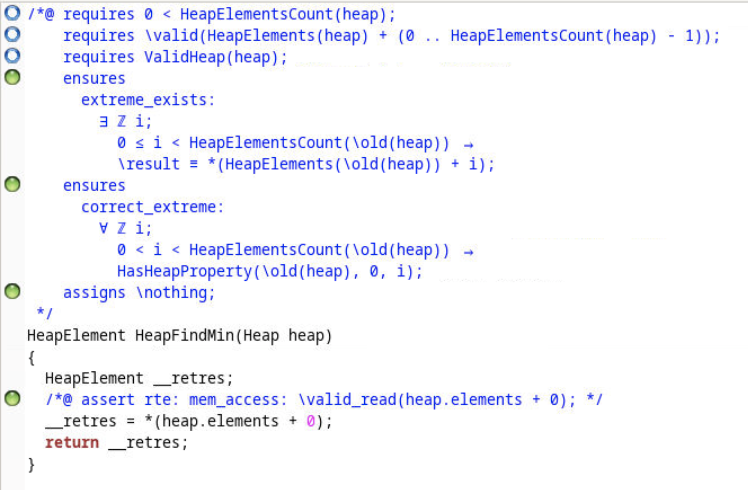
\includegraphics[width=10cm]{images/frama-c-HeapFindMin}
	\caption{Úspešné dokončení důkazu hledání minimálního prvku v prostředí Frama-C}
	\label{img:F-C-HeapFindMin}
\end{figure}

Na obrázku \ref{img:F-C-HeapFindMin} je vidět úspěšně dokončený důkaz korektnosti hledání minimálního prvku v haldě.

Ostatní funkce a anotace v implementaci binární haldy nevyužívají axiomy a lze dokázat jejich korektnost pomocí nástrojů \textit{alt-ergo} nebo \textit{cvc4}.

\section{Probublání prvku nahoru}
\label{subsec:HeapBubbleUp}

Probublání prvku haldy směrem nahoru (ke kořeni) je operace nad haldou, která dokáže v čase $\mathcal{O}(\log(n))$ opravit haldové uspořádání za předpokladu, že se snížila hodnota pouze toho vrcholu, který má být probublán.

Algoritmus předpokládá, že haldové uspořádání lze porušit pouze mezi jednou dvojicí vrcholů $u$ a $v$, kde $u$ je rodičovský vrchol a $v$ je jeho potomek. Tedy v celé haldě s výjimkou této dvojice musí platit haldové uspořádání. V této dvojici může platit, že syn~$v$ má menší hodnotu než jeho otec~$u$. Dále se předpokládá, že tento algoritmus bude proveden po zmenšení hodnoty některého vrcholu nebo po vložení nového vrcholu do haldy. V obou případech je potřeba tento vrchol probublat nahoru do správné pozice v haldě. Pokud by se hodnota zvýšila, měl by být aplikován algoritmus probublání dolů, o kterém pojednává sekce \ref{subsec:HeapBubbleDown}.

\begin{listing}[H]
	\caption{Probublání prvku nahoru}
	\label{list:HeapBubbleUp}
	\begin{minted}{c}
void HeapBubbleUp(Heap heap, int index) {
  int parent;

  while (HeapHasParent(heap, index)) {
    parent = HeapParent(index);

    if (HeapElementValue(heap, parent) <= HeapElementValue(heap, index)) {
      break;
    }

    HeapSwap(heap, index, parent);

    index = parent;
  }
}
	\end{minted}
\end{listing}

Pro důkaz korektnosti tohoto algoritmu jsou použity \textit{řezy} haldou. Tyto řezy slouží pro rozdělení grafu haldy na dva podgrafy, ve kterých platí haldové uspořádání. Řezy dohromady tvoří původní graf haldy bez jedné problematické hrany $(u, v)$, ve které nemusí platit haldové uspořádání.

Rozdělení haldy pro operaci probublání nahoru by mohlo vypadat podobně jak znázorňuje obrázek \ref{img:heap-intuitive-cut}. Tento přístup ale není vhodný pro algoritmické zpracování a dokazovaní, jelikož se toto rozdělení složitě popisuje. Zavedeme proto horní a spodní řezy haldy pomocí potomka, které pracují s indexy jednotlivých prvků haldy reprezentované polem.

\begin{figure}[H]
	\centering
	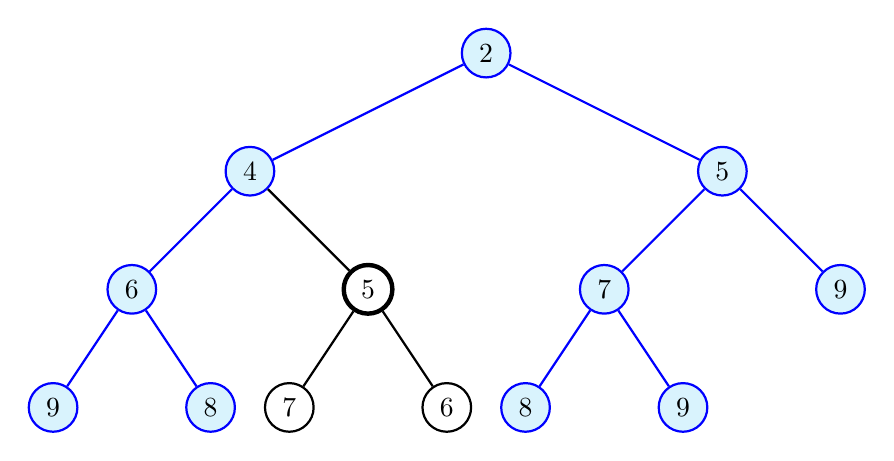
\begin{tikzpicture}[level/.style={sibling distance=60mm/#1}]
		\node [circle,thick,draw=blue,fill=cyan!15] (0) {2}
		child[thick,draw=blue] { node [circle,draw,fill=cyan!15] (1) {4}
			child { node [circle,draw,fill=cyan!15] (3) {6}
				child { node [circle,draw,fill=cyan!15] (7) {9} }
				child { node [circle,draw,fill=cyan!15] (8) {8} }
			}
			child[draw=black] { node [circle,draw,ultra thick] (4) {5}
				child { node [circle,draw] (9) {7} }
				child { node [circle,draw] (10) {6} }
			}
		}
		child[thick,draw=blue] { node [circle,draw,fill=cyan!15] (2) {5}
			child { node [circle,draw,fill=cyan!15] (5) {7}
				child { node [circle,draw,fill=cyan!15] (11) {8} }
				child { node [circle,draw,fill=cyan!15] (12) {9} }
			}
			child { node [circle,draw,fill=cyan!15] (6) {9} }
		};
	\end{tikzpicture}
	\caption{Ukázka intuitivního řezu haldy}
	\label{img:heap-intuitive-cut}
\end{figure}

\begin{definition}[Vrchní řez haldy pomocí potomka]
	Mějme graf $G = (V, E)$ reprezentující binární haldu a~$i \in \mathbb{N}$.
	Vrchním řezem haldy pomocí potomka nazveme graf $G' = (V', E')$, kde
	\begin{enumerate}
	  \item[] $V' = \{ v: v \in V \land \Index(v) < i \}$
	  \item[] $E' = \{ (u, v): (u, v) \in E \land u \in V' \land v \in V' \}$.
	\end{enumerate}
\end{definition}

\begin{figure}[H]
	\centering
	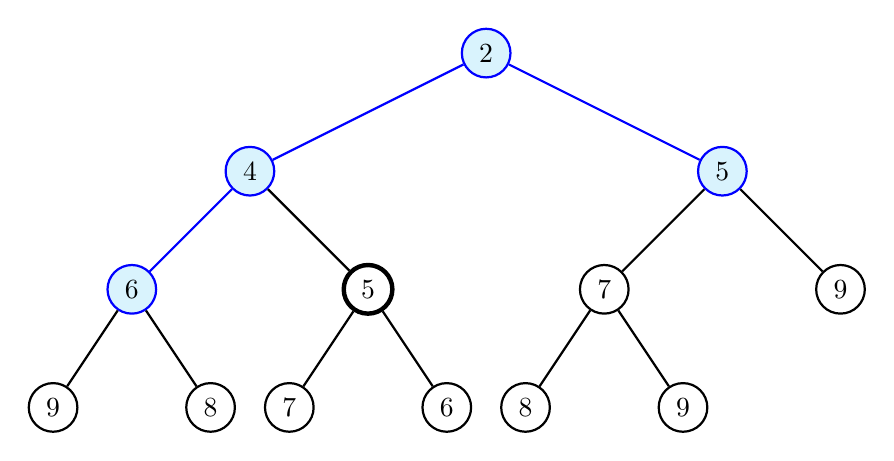
\begin{tikzpicture}[level/.style={sibling distance=60mm/#1}]
		\node [circle,thick,draw=blue,fill=cyan!15] (0) {2}
		child[thick,draw=blue] { node [circle,draw,fill=cyan!15] (1) {4}
			child { node [circle,draw,fill=cyan!15] (3) {6}
				child[draw=black] { node [circle,draw] (7) {9} }
				child[draw=black] { node [circle,draw] (8) {8} }
			}
			child[draw=black] { node [circle,draw,ultra thick] (4) {5}
				child { node [circle,draw] (9) {7} }
				child { node [circle,draw] (10) {6} }
			}
		}
		child[thick,draw=blue] { node [circle,draw,fill=cyan!15] (2) {5}
			child[draw=black] { node [circle,draw] (5) {7}
				child { node [circle,draw] (11) {8} }
				child { node [circle,draw] (12) {9} }
			}
			child[draw=black] {node [circle,draw] (6) {9} }
		};
	\end{tikzpicture}
	\caption{Ukázka vrchního řezu haldy pomocí potomka}
	\label{img:heap-upper-child-cut}
\end{figure}

\begin{remark}
	V grafu vrchního řezu haldy pomocí potomka platí haldové uspořádání.
\end{remark}

ACSL kód popisující vrchní řez haldy pomocí potomka nevytváří nový podgraf s~výše definovanými vlastnostmi, ale pouze ověřuje, že daná část (podgraf) haldy splňuje haldové uspořádání. Takto vytvořený predikát je následně použit v kontraktu funkce jako jedna ze vstupních podmínek algoritmu probublání nahoru a je také použit jako invariant cyklu. Predikát je tedy platný při volání funkce, po každém kroku cyklu a je také platný na konci vykonávání funkce. Tato induktivní vlastnost následně napomáhá při dokončení důkazu korektnosti algoritmu probublání nahoru. Nemusí ale platit, že graf vrchního řezu pomocí potomka je na konci vykonávání funkce prázdný. Tato situace nastává pouze v případě, když je problematický vrchol probublán do kořene haldy.

\begin{listing}[H]
	\caption{Predikát validního vrchního řezu v haldě pomocí potomka}
	\label{acsl:HeapUpperChildCut}
	\begin{minted}{c}
/*@
  predicate HeapUpperChildCut(Heap heap, integer index) =
    \forall integer ancestor, descendant;
      0 <= ancestor < descendant < HeapElementsCount(heap)
      && descendant < index
      && IsParent(ancestor, descendant) ==>
        HasHeapProperty(heap, ancestor, descendant);
*/
	\end{minted}
\end{listing}

\begin{definition}[Spodní řez haldy pomocí potomka]
	Mějme graf $G = (V, E)$ reprezentující binární haldu a~$i \in \mathbb{N}$.
	Spodním řezem haldy pomocí potomka nazveme graf $G' = (V', E')$, kde
	\begin{enumerate}
	  \item[] $V' = \{ v: v \in V \land \Index(v) > i \} \cup \{ \Parent(v): v \in V \land \Index(v) > i \}$
	  \item[] $E' = \{ (u, v): (u, v) \in E \land u \in V' \land v \in V' \}$.
	\end{enumerate}
\end{definition}

\begin{figure}[H]
	\centering
	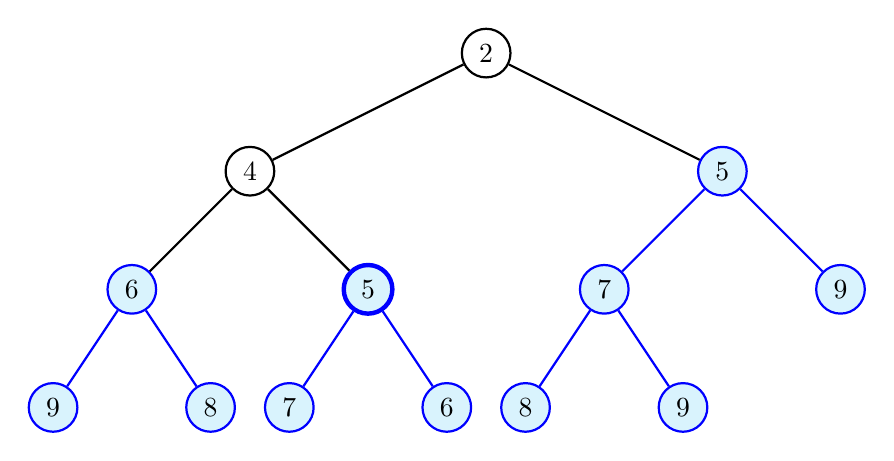
\begin{tikzpicture}[level/.style={sibling distance=60mm/#1}]
		\node [circle,thick,draw] (0) {2}
		child[thick] { node [circle,draw] (1) {4}
			child { node [circle,draw=blue,fill=cyan!15] (3) {6}
				child[draw=blue] { node [circle,draw,fill=cyan!15] (7) {9} }
				child[draw=blue] { node [circle,draw,fill=cyan!15] (8) {8} }
			}
			child { node [circle,draw=blue,fill=cyan!15,ultra thick] (4) {5}
				child[draw=blue] { node [circle,draw,fill=cyan!15] (9) {7} }
				child[draw=blue] { node [circle,draw,fill=cyan!15] (10) {6} }
			}
		}
		child[thick] { node [circle,draw=blue,fill=cyan!15] (2) {5}
			child[draw=blue] { node [circle,draw,fill=cyan!15] (5) {7}
				child { node [circle,draw,fill=cyan!15] (11) {8} }
				child { node [circle,draw,fill=cyan!15] (12) {9} }
			}
			child[draw=blue] {node [circle,draw,fill=cyan!15] (6) {9} }
		};
	\end{tikzpicture}
	\caption{Ukázka spodního řezu haldy pomocí potomka}\label{img:heap-lower-child-cut}
\end{figure}

\begin{remark}
	V grafu spodního řezu haldy pomocí potomka platí haldové uspořádání.
\end{remark}

ACSL predikát pro spodní řez haldy pomocí potomka je velmi podobný predikátu vrchního řezu haldy pomocí potomka. Pokrývá ale vrcholy haldy s indexem větším než problematický vrchol a jejich rodičovské vrcholy. Nemusí ale platit, že graf spodního řezu pomocí potomka na konci vykonávání obsahuje celou původní haldu. Tato situace nastává pouze v případě, když je problematický vrchol probublán do kořene haldy.

\begin{listing}[H]
	\caption{Predikát validního spodního řezu v haldě pomocí potomka}
	\label{acsl:HeapLowerChildCut}
	\begin{minted}{c}
/*@
  predicate HeapLowerChildCut(Heap heap, integer index) =
    \forall integer ancestor, descendant;
      0 <= ancestor < descendant < HeapElementsCount(heap)
      && index < descendant
      && IsParent(ancestor, descendant) ==>
        HasHeapProperty(heap, ancestor, descendant);
*/
	\end{minted}
\end{listing}

ACSL predikát \ref{acsl:HeapLowerChildCut} správně odděluje vrcholy, které mají index menší než problematický vrchol. Zároveň ale neomezuje hodnoty rodičovských vrcholů. Proto se do spodního řezu pomocí potomka správně dostane i problematický vrchol a také některé rodičovské vrcholy, které mají menší index než problematický vrchol. Hrana mezi problematickým vrcholem a jeho rodičovským vrcholem zde správně není.

Poslední nutnou vlastností pro úspěšné dokončení důkazu je tranzitivní haldové uspořádání mezi vrchním a spodním řezem haly. Tato vlastnost je automaticky splněna pro všechny hrany s výjimkou hrany, na které leží problematický vrchol v roli potomka. Proto do kódu zavádíme vstupní podmínku a invariantu cyklu, které kontrolují, zda platí haldové uspořádání pro rodičovský vrchol problematického vrcholu a jednotlivé potomky problematického vrcholu.

Tato vlastnost umožňuje probublávat problematický vrchol nahoru. Zaručuje totiž, že rodičovský prvek, který s problematickým vrcholem vyměníme, bude po provedení výměny splňovat haldové uspořádání se svými novými potomky.

\begin{listing}[H]
	\caption{Predikáty tranzitivního haldového uspořádání mezi řezy haldou}
	\begin{minted}{c}
/*@
  predicate HeapCutHeapPropertyLeftChild(Heap heap, integer index) = 
    HeapHasParent(heap, index)
    && HeapHasLeftChild(heap, index) ==>
      HasHeapProperty(heap, Parent(index), LeftChild(index));

  predicate HeapCutHeapPropertyRightChild(Heap heap, integer index) =
    HeapHasParent(heap, index)
    && HeapHasRightChild(heap, index) ==>
      HasHeapProperty(heap, Parent(index), RightChild(index));
*/
	\end{minted}
\end{listing}

Platnost těchto čtyř invariantů dokazuje, že algoritmus probublání nahoru vždy vytváří maximálně jednu novou problematickou dvojici vrcholů. Haldové uspořádání mezi touto dvojicí vrcholů je opraveno probubláním na správnou pozici nebo úplným probubláním vrcholu do kořene haldy.

Spojením horního a spodního řezu haldou a tranzitivního haldového uspořádání je možné formálně dokázat korektnost algoritmu probublání prvku nahoru. Jelikož tyto vlastnosti platí na konci každého kroku cyklu, po dokončení cyklu se nacházíme v jednom z těchto stavů:

\begin{enumerate}
  \item problematický prvek probublal až do kořene haldy,
  \item problematický prvek nemohl dále probublat, tudíž je na správné pozici v haldě.
\end{enumerate}

Oba případy nám při spojení znalostí o horním a dolním řezu pomocí potomka a znalostí o aktuálně opravené hraně dávají výsledek, že pro každou hranu $(u, v)$ haldy, kde $u$ je rodičovský vrchol $v$, platí haldové uspořádání.

\begin{figure}[H]
	\centering
	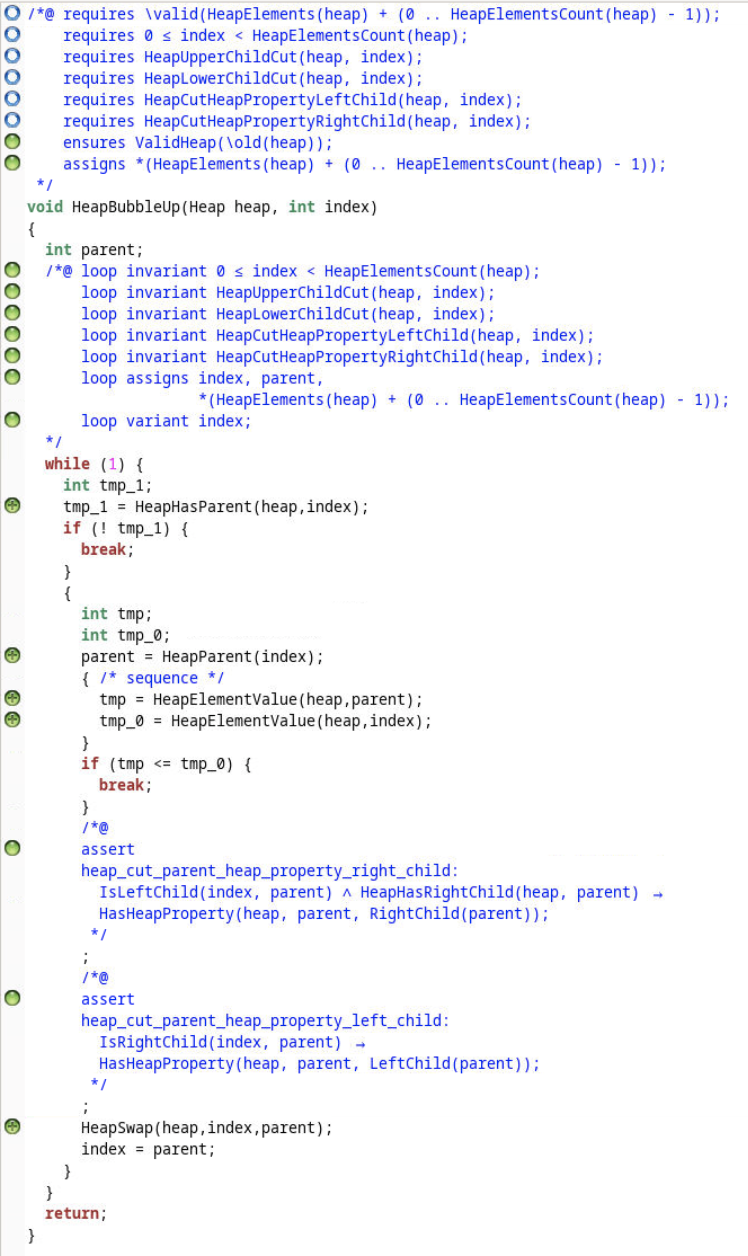
\includegraphics[width=10cm]{images/frama-c-HeapBubbleUp}
	\caption{Úspešné dokončení důkazu probublání nahoru v prostředí Frama-C}
	\label{img:F-C-HeapBubbleUp}
\end{figure}

\section{Vložení prvku}
\label{subsec:HeapInsert}

Vložení prvku do haldy je operace nad haldou, která v čase $\mathcal{O}(1)$ vloží nový vrchol do haldy a následně v~čase $\mathcal{O}(\log(n))$ tento vrchol umístí na správnou pozici v haldě. Celková asymptotická časová složitost je tedy $\mathcal{O}(\log(n))$.

Algoritmus přidává nový vrchol do nejspodnější hladiny haldy tak, aby byl udržen tvar haldy. Pro takto vložený vrchol ale nemusí platit haldové uspořádání s jeho rodičovským vrcholem. Mohlo se stát, že vložený vrchol má menší hodnotou než jeho rodičovský vrchol. Proto je nutné provést probublání nahoru, o kterém pojednává sekce \ref{subsec:HeapBubbleUp}.

Algoritmus probublání vrcholu nahoru má tři vstupní podmínky. V haldě musí platit predikát o horním řezu podle potomka, který v případě přidání nového vrcholu platí. Před přidáním vrcholu byla halda validní a platilo v ní haldové uspořádání. Nový prvek je vložen na nový největší index v haldě. Tedy pro tento nový index platí vrchní řez haldou pomocí potomka, protože tento řez popisuje původní haldu, ve které platilo haldové uspořádání. Spodní řez haldy pomocí potomka také platí, protože se jedná o prázdný graf. Tranzitivní haldové uspořádání u aktuálně přidaného vrcholu také platí, protože tento vrchol nemá žádné potomky.

\begin{figure}[H]
	\centering
	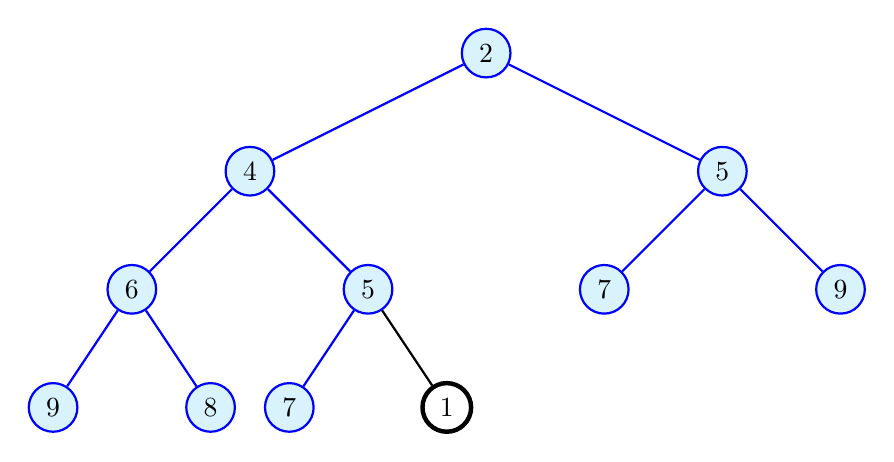
\begin{tikzpicture}[level/.style={sibling distance=60mm/#1}]
		\node [circle,thick,draw=blue,fill=cyan!15] (0) {2}
		child[thick,draw=blue] { node [circle,draw,fill=cyan!15] (1) {4}
			child { node [circle,draw,fill=cyan!15] (3) {6}
				child { node [circle,draw,fill=cyan!15] (7) {9} }
				child { node [circle,draw,fill=cyan!15] (8) {8} }
			}
			child { node [circle,draw,,fill=cyan!15] (4) {5}
				child { node [circle,draw,fill=cyan!15] (9) {7} }
				child[draw=black] { node [circle,draw,ultra thick] (10) {1} }
			}
		}
		child[thick,draw=blue] { node [circle,draw,fill=cyan!15] (2) {5}
			child { node [circle,draw,fill=cyan!15] (5) {7} }
			child { node [circle,draw,fill=cyan!15] (6) {9} }
		};
	\end{tikzpicture}
	\caption{Ukázka vrchního řezu haldy pomocí potomka při přidání vrcholu}\label{img:heap-insert-heap-upper-child-cut}
\end{figure}

Na obrázku \ref{img:heap-insert-heap-upper-child-cut} je zobrazeno přidání nového vrcholu do haldy a je zvýrazněn horní řez haldy podle potomka.

Algoritmus probublání nahoru tento nový vrchol vymění s jeho rodičovským vrcholem, protože nově přidaný vrchol má menší hodnotu než jeho rodičovský vrchol. Tímto prvním krokem algoritmu se nově přidaný vrchol dostal níže v haldě, ale stále platí všechny tři invarianty cyklu. Horní řez haldy pomocí potomka se pouze zmenšil a spodní řez haldy pomocí potomka se zvětšil o vrcholy, které se v původním kroku vyskytovaly v horním řezu a také o vrchol původního rodiče nového vrcholu. Tranzitivní haldové uspořádání začíná platit mezi rodičovským prvkem aktuálně probublaného vrcholu a jeho potomky.

Algoritmem probublání se nový vrchol dostane do správné pozice a ve výsledné haldě, o jeden vrchol větší, je opraveno haldové uspořádání.

\begin{listing}[H]
	\caption{Vložení prvku}
	\label{list:HeapInsert}
	\begin{minted}{c}
/*@
    requires 0 <= HeapElementsCount(heap) < HeapElementsCapacity(heap);
    requires \valid(HeapElements(heap) + (0 .. HeapElementsCapacity(heap) - 1));
    requires ValidHeap(heap);
    requires correctly_indexed:
    	HeapElementIndex(element) == HeapElementsCount(heap);

    assigns HeapElements(heap)[0..HeapElementsCount(heap)];
    
    ensures count_increase: 
    	HeapElementsCount(\result) == HeapElementsCount(heap) + 1;
    ensures ValidHeap(\result);
*/
Heap HeapInsert(Heap heap, HeapElement element) {
  int index = heap.elementsCount;

  heap.elements[index] = element;
  heap.elementsCount++;

  HeapBubbleUp(heap, index);

  return heap;
}
	\end{minted}
\end{listing}

ACSL anotace algoritmu probublání nahoru zajišťují, že po dokončení algoritmu je předaná halda validní. Haldové uspořádání tedy po dokončení probublání nahoru platí v celé haldě. Jelikož je volání probublání nahoru poslední akcí algoritmu vložení prvku, lze toto ujištění validnosti haldy vložit také do anotace algoritmu vkládání prvku. Tímto je zaručena korektnost algoritmu vkládání prvku do haldy.

\begin{figure}[H]
	\centering
	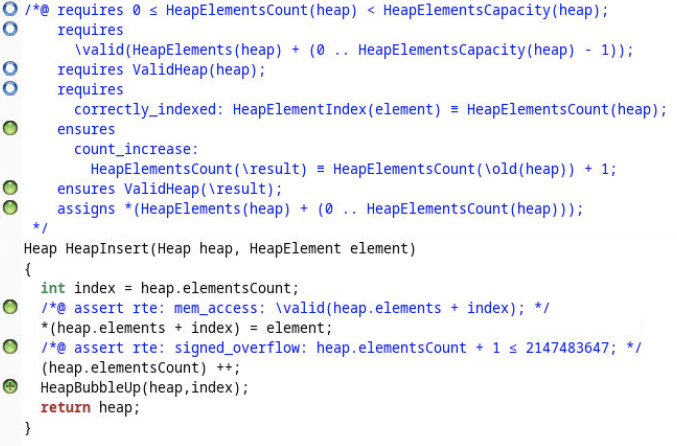
\includegraphics[width=10cm]{images/frama-c-HeapInsert}
	\caption{Úspešné dokončení důkazu vložení prvku do haldy v prostředí Frama-C}
	\label{img:F-C-HeapInsert}
\end{figure}


\section{Probublání prvku dolů}
\label{subsec:HeapBubbleDown}

Probublání prvku haldy směrem dolů (od kořene) je operace nad haldou, která dokáže v čase $\mathcal{O}(\log(n))$ opravit haldové uspořádání za předpokladu, že se zvýšila hodnota pouze toho vrcholu, která má být probublán.

Algoritmus předpokládá, že haldové uspořádání lze porušit maximálně u dvou dvojic vrcholů $u$ a $v$ nebo $u$ a $w$, kde $u$ je rodičovský vrchol vrcholů $v$ a $w$. Tedy v celé haldě s výjimkou těchto dvou dvojic musí platit haldové uspořádání. V těchto dvojicích může platit, že rodič~$u$~má větší hodnotu než některý z jeho potomků. Může nastat situace, kdy rodičovský vrchol~$u$~má větší hodnotu než oba jeho potomci. Dále se předpokládá, že tento algoritmus bude proveden po zvětšení hodnoty některého vrcholu nebo při vytváření haldy. V obou případech je potřeba tento vrchol probublat dolů do správné pozice v haldě. Pokud by se hodnota snížila, měl by být aplikován algoritmus probublání nahoru, o kterém pojednává sekce \ref{subsec:HeapBubbleUp}.


\begin{listing}[H]
	\caption{Probublání prvku dolů}
	\label{list:HeapBubbleDown}
	\begin{minted}{c}
void HeapBubbleDown(Heap heap, int index) {
    int child;

    while (HeapHasChild(heap, index)) {
        child = HeapLowerChild(heap, index);

        if (HeapElementValue(heap, index) <= HeapElementValue(heap, child)) {
            break;
        }

        HeapSwap(heap, index, child);

        index = child;
    }
}
	\end{minted}
\end{listing}

Pro důkaz korektnosti tohoto algoritmu jsou požity \textit{řezy} haldou, podobné řezům použitých pro důkaz korektnosti probublání nahoru popsané v sekci \ref{subsec:HeapBubbleUp}. Řezy haldou pro důkaz probublání dolů jsou mírně odlišné od řezů v důkazu korektnosti algoritmu probublání nahoru, jelikož řezy haldou pomocí rodiče povolují až dvě problematické hrany v haldě.

\begin{definition}[Vrchní řez haldy pomocí rodiče]
	Mějme graf $G = (V, E)$ reprezentující binární haldu a~$i \in \mathbb{N}$.
	Vrchním řezem haldy pomocí rodiče nazveme graf $G' = (V', E')$, kde
	\begin{enumerate}
	  \item[] $V' = \{ v: v \in V \land \Index(v) < i \} \cup \{ \LeftChild(v): v \in V \land \Index(v) < i \} \cup \{ \RightChild(v): v \in V \land \Index(v) < i \}$
	  \item[] $E' = \{ (u, v): (u, v) \in E \land u \in V' \land v \in V' \}$.
	\end{enumerate}
\end{definition}

\begin{figure}[H]
	\centering
	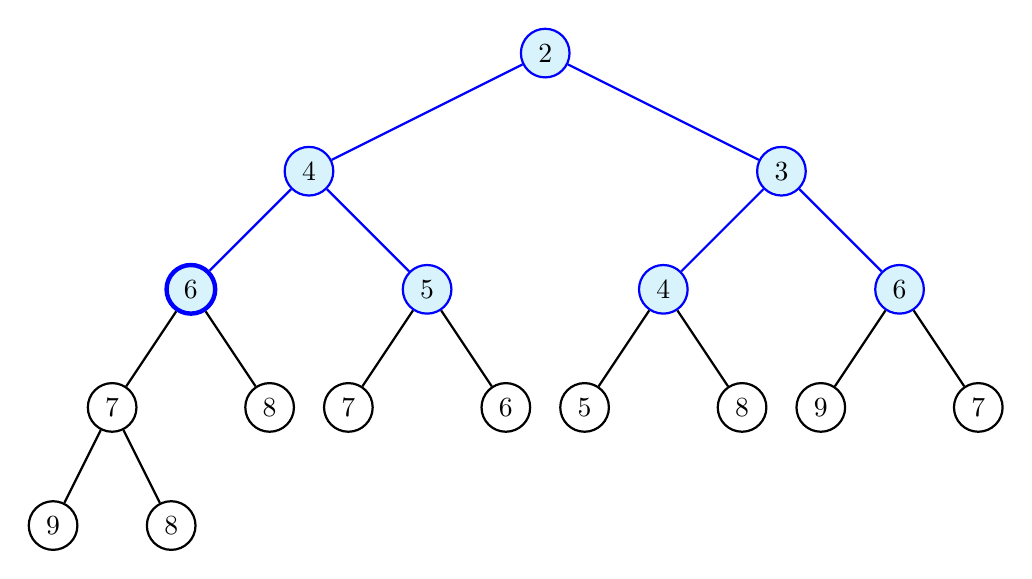
\begin{tikzpicture}[level/.style={sibling distance=60mm/#1}]
		\node [circle,thick,draw=blue,fill=cyan!15] (0) {2}
		child[thick,draw=blue] { node [circle,draw,fill=cyan!15] (1) {4}
			child { node [circle,draw,ultra thick,fill=cyan!15] (3) {6}
				child[draw=black] { node [circle,draw] (7) {7} 
					child { node [circle,draw] (15) {9} }
					child { node [circle,draw] (16) {8} }				
				}
				child[draw=black] { node [circle,draw] (8) {8} }
			}
			child { node [circle,draw,fill=cyan!15] (4) {5}
				child[draw=black] { node [circle,draw] (9) {7} }
				child[draw=black] { node [circle,draw] (10) {6} }
			}
		}
		child[thick,draw=blue] { node [circle,draw,fill=cyan!15] (2) {3}
			child { node [circle,draw,fill=cyan!15] (5) {4}
				child[draw=black] { node [circle,draw] (11) {5} }
				child[draw=black] { node [circle,draw] (12) {8} }
			}
			child { node [circle,draw,fill=cyan!15] (7) {6}
				child[draw=black] { node [circle,draw] (13) {9} }
				child[draw=black] { node [circle,draw] (14) {7} }
			}
		};
	\end{tikzpicture}
	\caption{Ukázka vrchního řezu haldy pomocí rodiče}\label{img:heap-upper-parent-cut}
\end{figure}

\begin{remark}
	V grafu vrchního řezu haldy pomocí rodiče platí haldové uspořádání.
\end{remark}

ACSL kód popisující vrchní řez haldy pomocí rodiče nevytváří nový podgraf s~výše definovanými vlastnostmi, ale pouze ověřuje, že daná část (podgraf) haldy splňuje haldové uspořádání. Takto vytvořený predikát je následně použit v kontraktu funkce jako jedna ze vstupních podmínek algoritmu probublání dolů a je také použit jako invariant cyklu. Predikát je tedy platný při volání funkce, po každém kroku cyklu a je také platný na konci vykonávání funkce. Nemusí ale platit, že graf vrchního řezu pomocí rodiče na konci vykonávání funkce obsahuje celou původní haldu. Tato situace nastává pouze v případě, když je problematický vrchol probublán do vrcholu s maximálním indexem v haldě. Tato induktivní vlastnost následně napomáhá při dokončení důkazu korektnosti algoritmu probublání dolů.

\begin{listing}[H]
	\caption{Predikát validního vrchního řezu v haldě pomocí rodiče}
	\label{acsl:HeapUpperParentCut}
	\begin{minted}{c}
/*@
  predicate HeapUpperParentCut(Heap heap, integer index) =
    \forall integer ancestor, descendant;
      0 <= ancestor < index
      && ancestor < descendant < HeapElementsCount(heap)
      && IsParent(ancestor, descendant) ==>
        HasHeapProperty(heap, ancestor, descendant);
*/
	\end{minted}
\end{listing}

\begin{definition}[Spodní řez haldy pomocí rodiče]
	Mějme graf $G = (V, E)$ reprezentující binární haldu a~$i \in \mathbb{N}$.
	Spodním řezem haldy pomocí rodiče nazveme graf $G' = (V', E')$, kde
	\begin{enumerate}
	  \item[] $V' = \{ v: v \in V \land \Index(v) > i \}$
	  \item[] $E' = \{ (u, v): (u, v) \in E \land u \in V' \land v \in V' \}$.
	\end{enumerate}
\end{definition}

\begin{figure}[H]
	\centering
	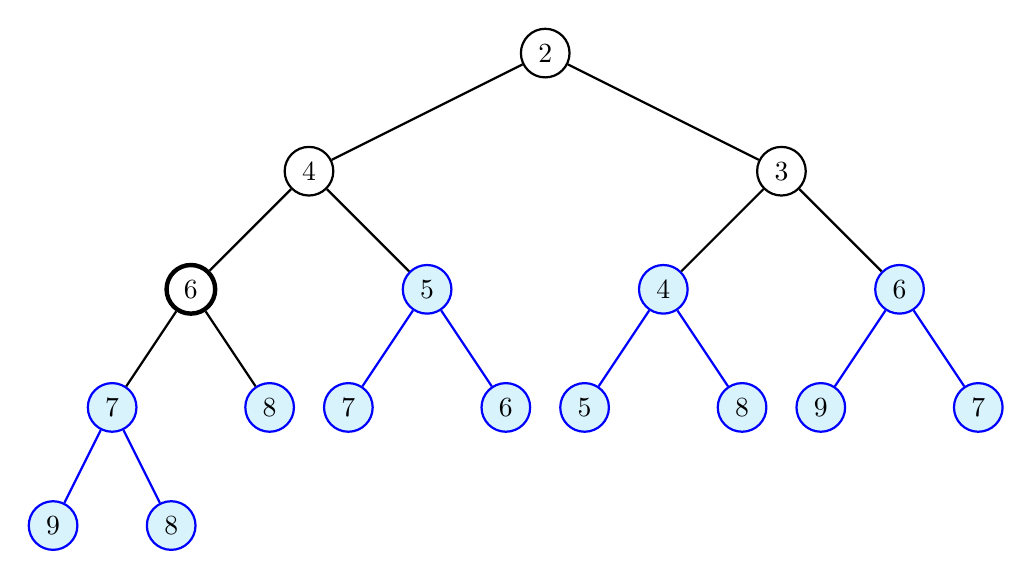
\begin{tikzpicture}[level/.style={sibling distance=60mm/#1}]
		\node [circle,draw,thick] (0) {2}
		child[thick] { node [circle,draw] (1) {4}
			child { node [circle,draw,ultra thick] (3) {6}
				child { node [circle,draw=blue,fill=cyan!15] (7) {7} 
					child[draw=blue] { node [circle,draw,fill=cyan!15] (15) {9} }
					child[draw=blue] { node [circle,draw,fill=cyan!15] (16) {8} }				
				}
				child { node [circle,draw=blue,fill=cyan!15] (8) {8} }
			}
			child { node [circle,draw=blue,fill=cyan!15] (4) {5}
				child[draw=blue] { node [circle,draw,fill=cyan!15] (9) {7} }
				child[draw=blue] { node [circle,draw,fill=cyan!15] (10) {6} }
			}
		}
		child[thick] { node [circle,draw] (2) {3}
			child { node [circle,draw=blue,fill=cyan!15] (5) {4}
				child[draw=blue] { node [circle,draw,fill=cyan!15] (11) {5} }
				child[draw=blue] { node [circle,draw,fill=cyan!15] (12) {8} }
			}
			child { node [circle,draw=blue,fill=cyan!15] (7) {6}
				child[draw=blue] { node [circle,draw,fill=cyan!15] (13) {9} }
				child[draw=blue] { node [circle,draw,fill=cyan!15] (14) {7} }
			}
		};
	\end{tikzpicture}
	\caption{Ukázka spodního řezu haldy pomocí rodiče}\label{img:heap-lower-parent-cut}
\end{figure}

\begin{remark}
	V grafu spodního řezu haldy pomocí rodiče platí haldové uspořádání.
\end{remark}

ACSL predikát pro spodní řez haldy pomocí rodiče je velmi podobný predikátu vrchního řezu haldy pomocí rodiče. Pokrývá ale vrcholy haldy s indexem větším než problematický vrchol. Nemusí ale platit, že graf spodního řezu pomocí rodiče je na konci vykonávání funkce prázdný. Tato situace nastává pouze v případě, když je problematický vrchol probublán do vrcholu s maximálním indexem v haldě.

\begin{listing}[H]
	\caption{Predikát validního spodního řezu v haldě pomocí rodiče}
	\label{acsl:HeapLowerParentCut}
	\begin{minted}{c}
/*@
  predicate HeapLowerParentCut(Heap heap, integer index) =
    \forall integer ancestor, descendant;
      index < ancestor < HeapElementsCount(heap)
      && ancestor < descendant < HeapElementsCount(heap)
      && IsParent(ancestor, descendant) ==>
        HasHeapProperty(heap, ancestor, descendant);
*/
	\end{minted}
\end{listing}

Algoritmus probublání dolů je v binární haldě aplikován po zvýšení hodnoty některého vrcholu nebo při rychlé konstrukci haldy, o které pojednává sekce \ref{subsec:HeapBuild}. Při zvýšení hodnoty vrcholu můžeme využít horní a dolní řez haldou pomocí rodiče a pomocí invariantů cyklu formálně dokázat korektnosti algoritmu.

Problém představuje algoritmus rychlé konstrukce haldy. Tento algoritmu postupně probublává dolů rodičovské vrcholy od vrcholu s největším indexem až po index kořene haldy. Při tomto způsobu konstrukce je haldové uspořádání zaručeno pouze v dolním řezu haldy pomocí rodiče.

ACSL anotace funkce probublání dolů může přijímat dva typy vstupních dat. Základní vstup musí splňovat pouze predikát o spodním řezu haldou pomocí rodiče. V tomto případě algoritmus probublání zajišťuje pouze částečné opravení haldy. Zajišťuje zvětšení podgrafu dolního řezu haldou pomocí rodiče právě o probublávaný vrchol. Tato vlastnost je vhodná pro využití v invariantu cyklu algoritmu rychlé konstrukce haldy, jelikož zajišťuje postupné opravovaní haldového uspořádání.

Druhý typ vstupu je striktnější. Jedná se o vstup, ve kterém musí platit podmínky základního vstupu, tedy predikát spodního řezu haldou pomocí rodiče ale zároveň musí platit také predikát vrchního řezu haldou pomocí rodiče a tranzitivní haldové uspořádání mezi těmi dvěma řezy. V tomto případě může algoritmus probublání dolů za pomoci invariantu cyklu dokázat, že po dokončení cyklu v celé haldě platí haldové uspořádání. Tento typ vstupu je využíván při zvýšení hodnoty vrcholu, jelikož zvýšením hodnoty jsme neporušili haldové uspořádání v horním řezu haldou pomocí rodiče ani v spodním řezu haldou pomocí rodiče.

Základní i striktní typ vstupu je možné dokázat najednou pomocí ACSL konstrukce \textit{behavior}, která umožňuje některé invarianty cyklu dokazovat pouze za předpokladu, že byl algoritmus zavolán s platným predikátem horního řezu haldou pomocí rodiče.

\begin{figure}[H]
	\centering
	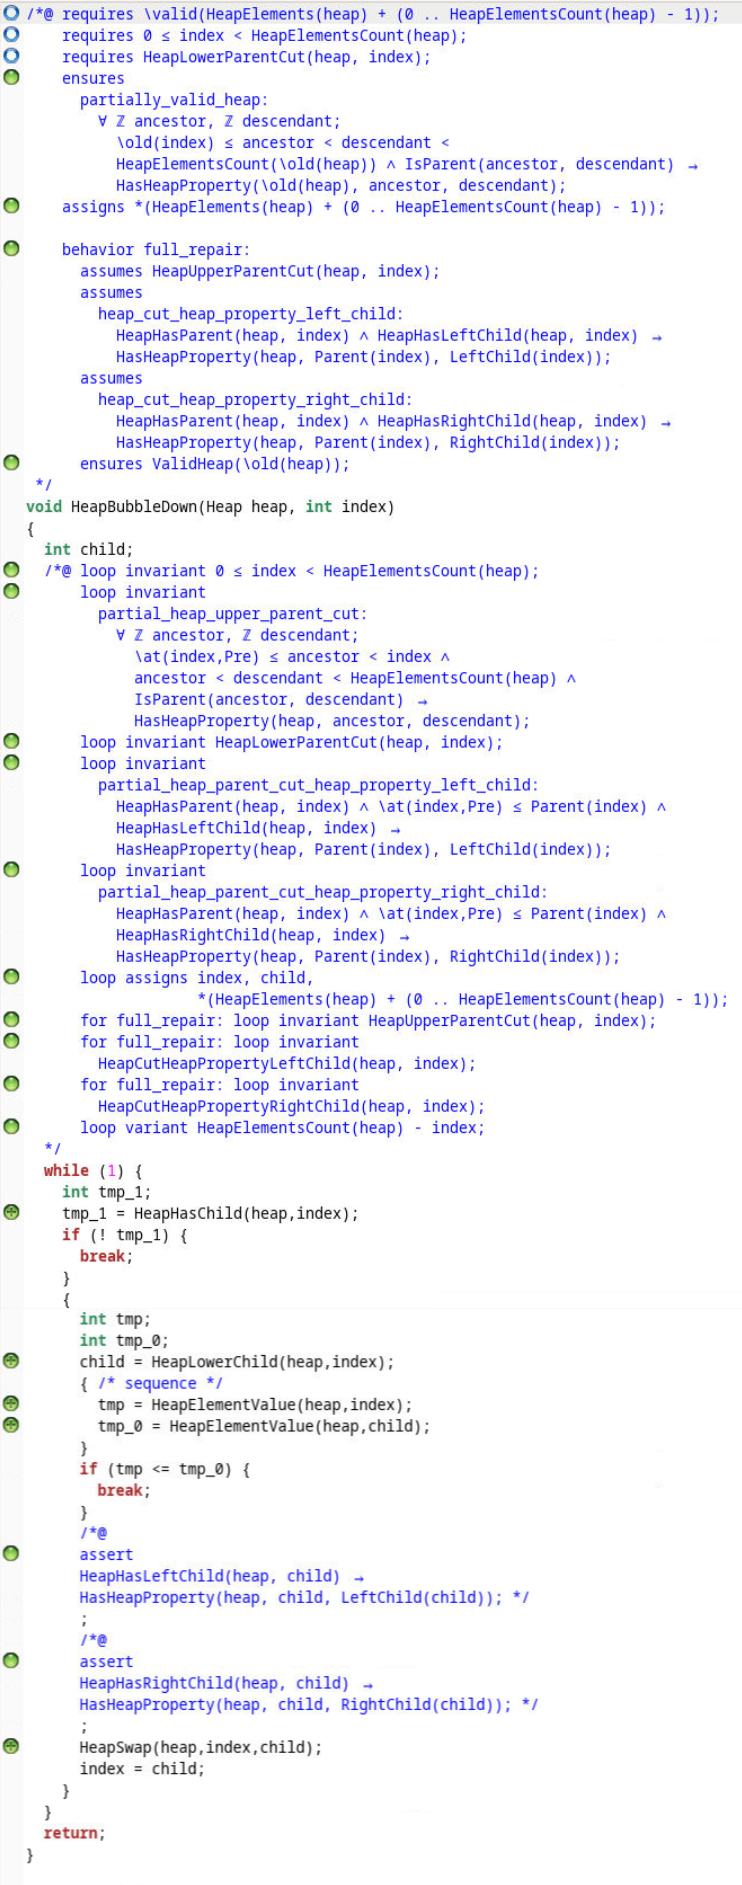
\includegraphics[width=9cm]{images/frama-c-HeapBubbleDown}
	\caption{Úspešné dokončení důkazu probublání dolů v prostředí Frama-C}
	\label{img:F-C-HeapBubbleDown}
\end{figure}

\section{Odstranění minimálního prvku}
\label{subsec:HeapExtractMin}

Datová struktura halda slouží jako prioritní fronta. Kořen haldy vždy obsahuje vrchol s nejmenší hodnotou. Algoritmy, které haldu využívají jako prioritní frontu, potřebují tento minimální prvek najít a odstranit z fronty. Hledání minimálního prvku zajišťuje algoritmus popsaný v sekci \ref{subsec:HeapFindMin}. Algoritmus odstranění minimálního prvku a důkaz korektnosti je popsán v této sekci.

Odstranění minimálního prvku z haldy je operace nad haldou, která v čase $\mathcal{O}(1)$ odstraní daný vrchol z haldy a v čase $\mathcal{O}(\log(n))$ opraví haldové uspořádání. Celková asymptotická časová složitost je tedy $\mathcal{O}(\log(n))$.

Kořen haldy lze bezproblémově odstranit pouze v případě, když je kořen jediný prvek v haldě. Pokud má kořen nějaké potomky, odstraněním kořene by se porušil tvar haldy.

\begin{remark}
Z haldy lze odstranit prvek s největším indexem, bez toho, aby se porušil tvar haldy.
\end{remark}

Algoritmus v prvním kroku vymění hodnotu uleženou v kořeni haldy s hodnotou uloženou ve vrcholu s největším indexem. Ve druhém kroku vrchol s největším indexem odstraní z haldy. Poslední krok algoritmu je probublání dolů kořene haldy.

Výměnou hodnoty v kořeni haldy a na největším indexu mohlo dojít k porušení haldového uspořádání. Algoritmus probublání má tři vstupní podmínky, pokud chceme získat haldové uspořádání v celé haldě. Horní řez haldou pomocí rodiče je triviálně splněn, jelikož se v případě probublání kořene jedná o prázdný graf. Spodní řez haldou obsahuje všechny vrcholy bez kořene a všechny hrany, na kterých neleží kořen. Jelikož v původní haldě před výměnou hodnoty kořene za hodnotu z vrcholu s největším indexem platilo haldové uspořádání, v podgrafu vytvořeným spodním řezem pomocí rodiče musí platit haldové uspořádání také. Tranzitivní haldové uspořádání triviálně platí, jelikož kořen nemá žádného rodiče.

\begin{figure}[H]
	\centering
	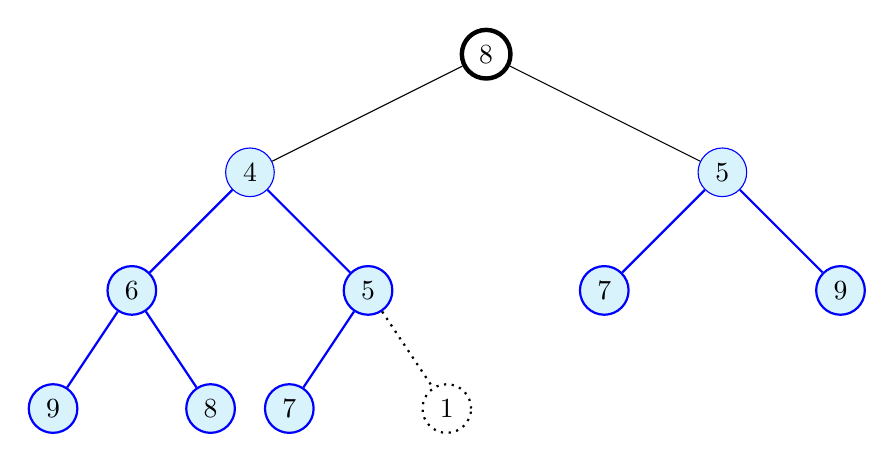
\begin{tikzpicture}[level/.style={sibling distance=60mm/#1}]
		\node [circle,draw,ultra thick] (0) {8}
		child { node [circle,draw=blue,fill=cyan!15] (1) {4}
			child[thick,draw=blue] { node [circle,draw,fill=cyan!15] (3) {6}
				child { node [circle,draw,fill=cyan!15] (7) {9} }
				child { node [circle,draw,fill=cyan!15] (8) {8} }
			}
			child[thick,draw=blue] { node [circle,draw,,fill=cyan!15] (4) {5}
				child { node [circle,draw,fill=cyan!15] (9) {7} }
				child[draw=black,dotted] { node [circle,draw] (10) {1} }
			}
		}
		child { node [circle,draw=blue,fill=cyan!15] (2) {5}
			child[thick,draw=blue] { node [circle,draw,fill=cyan!15] (5) {7} }
			child[thick,draw=blue] { node [circle,draw,fill=cyan!15] (6) {9} }
		};
	\end{tikzpicture}
	\caption{Ukázka spodního řezu haldy pomocí rodiče v průběhu odstraňování minimálního prvku}
	\label{img:heap-extract-min-heap-lower-parent-cut}
\end{figure}

Obrázek \ref{img:heap-extract-min-heap-lower-parent-cut} zobrazuje stav haldy po výměně hodnoty v kořeni za hodnotu ve vrcholu s~největším indexem. Tečkovaně je naznačena hrana a vrchol, které se v rámci algoritmu odstraňují a tučně je zvýrazněn nový kořen haldy, který bude v následujícím kroku algoritmu probublán dolů.

\begin{listing}[H]
	\caption{Kód a ACSL anotace odstranění minimálního prvku z haldy}
	\label{code:HeapExtractMin}
	\begin{minted}{c}
/*@
  requires 0 < HeapElementsCount(heap);
  requires \valid(HeapElements(heap) + (0 .. HeapElementsCount(heap) - 1));
  requires ValidHeap(heap);

  assigns HeapElements(heap)[0 .. HeapElementsCount(heap) - 1];

  ensures count_decrease: HeapElementsCount(\result) == HeapElementsCount(heap) - 1;
  ensures ValidHeap(\result);
*/
Heap HeapExtractMin(Heap heap) {
  int last = heap.elementsCount - 1;

  HeapSwap(heap, 0, last);

  heap.elementsCount--;

  if (0 < heap.elementsCount) {
    HeapBubbleDown(heap, 0);
  }

  return heap;
}
	\end{minted}
\end{listing}

Výpis kódu \ref{code:HeapExtractMin} zobrazuje kompletní kód odstranění minimálního prvku z haldy společně s ACSL anotacemi. Vstupní podmínka pro volání funkce odstranění minimálního prvku je nenulový počet prvků v haldě a haldové uspořádání v haldě. Výstupní anotace zajišťují, že funkce zmenšuje počet prvků v haldě a také, že ve zmenšené haldě stále platí haldové uspořádání.

Implementace tohoto algoritmu odhalila, že pro volání probublání dolů kořene je nutné v haldě po odstranění prvku s maximálním indexem alespoň jeden prvek stále mít. Některé pseudokódy tento krok nezohledňují. Tato chyba byla pomocí ACSL odhalena a bylo ji možné ihned opravit a dokončit důkaz korektnosti. Obrázek \ref{img:F-C-HeapExtractMin} zobrazuje úspěšně dokončený důkaz korektnosti algoritmu odstranění minimálního prvku z haldy.

\begin{figure}[H]
	\centering
	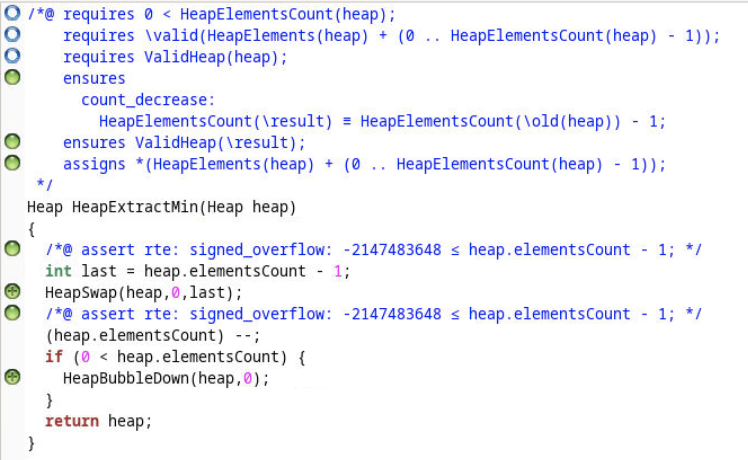
\includegraphics[width=10cm]{images/frama-c-HeapExtractMin}
	\caption{Úspešné dokončení důkazu odstranění minimálního prvku z haldy v prostředí Frama-C}
	\label{img:F-C-HeapExtractMin}
\end{figure}


\section{Změna hodnoty prvku}
\label{subsec:HeapChange}

Algoritmy, které využívají binární minimovou haldu mohou měnit hodnotu jednotlivých vrcholů haldy. Jedná se o změnu priority prvku, který je v haldě jednoznačně identifikovatelný. Funkce pro změnu hodnoty využívá dvě oddělené funkce, funkci pro snížení hodnoty vrcholu a funkci pro zvýšení hodnoty vrcholu.

\begin{listing}[H]
	\caption{Kód a ACSL anotace změny hodnoty prvku haldy}
	\label{code:HeapChange}
	\begin{minted}{c}
/*@
  requires \valid(HeapElements(heap) + (0 .. HeapElementsCount(heap) - 1));
  requires 0 <= index < HeapElementsCount(heap);
  requires ValidHeap(heap);

  assigns HeapElements(heap)[0 .. HeapElementsCount(heap) - 1];

  ensures value_changed:
    \exists integer i;
      0 <= i < HeapElementsCount(heap) ==>
        HeapElementValue(element) == HeapElementValue(heap, i);
  ensures ValidHeap(heap);
*/
void HeapChange(Heap heap, int index, HeapElement element) {
  if (_HeapElementValue(element) < HeapElementValue(heap, index)) {
    HeapDecrease(heap, index, element);
    return;
  }

  HeapIncrease(heap, index, element);
}
	\end{minted}
\end{listing}

Výpis kódu \ref{code:HeapChange} zobrazuje tělo funkce, která pomocí kontroly aktuální hodnoty vrcholu v haldě a požadované nové hodnotě prvku volá funkci pro zmenšení hodnoty prvku nebo zvětšení hodnoty prvku. Obě zmíněné funkce zajišťují změnu hodnoty vrcholu haldy a následné opravení haldového uspořádání, které se mohlo narušit změnou hodnoty prvku. Jelikož je volání těchto funkcí poslední akce ve funkci pro změnu hodnoty prvku v haldě, lze přidat stejné anotace pro ujištění o změně hodnoty prvku a opravení haldového uspořádání do anotace funkce o změně hodnoty prvku v haldě.

\begin{figure}[H]
	\centering
	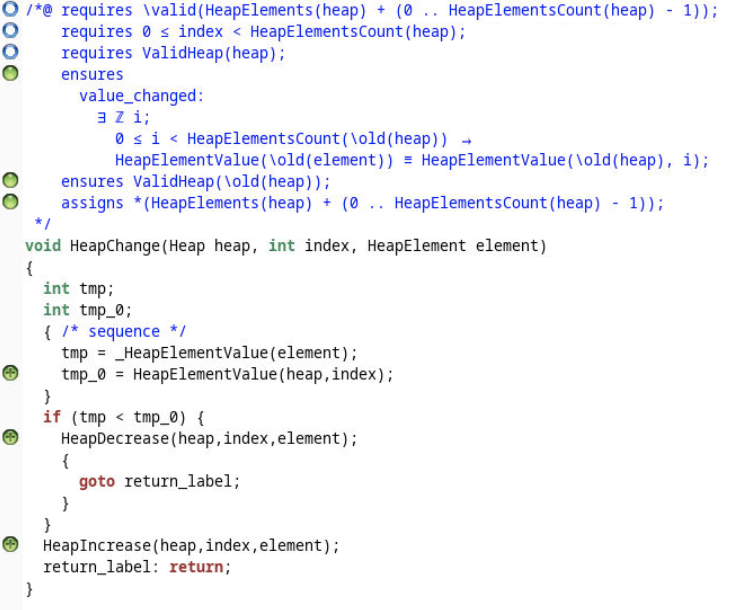
\includegraphics[width=10cm]{images/frama-c-HeapChange}
	\caption{Úspešné dokončení důkazu změny hodnoty prvku haldy v prostředí Frama-C}
	\label{img:F-C-HeapChange}
\end{figure}

Výpis kódu \ref{code:HeapChange} zobrazuje úspěšné dokončení důkazu korektnosti funkce pro změnu hodnoty prvku v haldě. Následné je vhodné dokázat korektnost jednotlivých funkcí pro snížení hodnoty prvku v haldě a pro zvýšení prvku v haldě.

\begin{listing}[H]
	\caption{Datová struktura prvku haldy}
	\label{code:HeapElement}
	\begin{minted}{c}
typedef struct _HeapElement {
  int index;

  int id;
  int value;
} HeapElement;
	\end{minted}
\end{listing}

Výpis kódu \ref{code:HeapElement} zobrazuje datovou strukturu prvky haldy. Tato struktura mimo jiné obsahuje aktuálním informaci o indexu daného prvku v haldě, na kterém je daný prvek uložen. Znalost indexu daného prvku umožňuje rychlý přístup k danému prvku v haldě implementované pomocí pole. Úpravu vrcholu je možné provést v čase $\mathcal{O}(1)$ pomocí přímého přístupu na index pole bez nutnosti daný prvek v haldě vyhledávat. 

Aktuální informace o indexu daného prvku v haldě je automaticky aktualizována při jakékoli změně či prohození dvou prvků v haldě, jak je znázorněno na výpisu kódu \ref{code:HeapSwap}.

\begin{listing}[H]
	\caption{Kód a ACSL anotace prohození dvou prvků v hladě}
	\label{code:HeapSwap}
	\begin{minted}{c}
/*@
  requires 0 <= a < HeapElementsCount(heap);
  requires 0 <= b < HeapElementsCount(heap);
  requires \valid(HeapElements(heap) + a);
  requires \valid(HeapElements(heap) + b);

  assigns HeapElements(heap)[a], HeapElements(heap)[b];

  ensures indexes_swapped_a:
    HeapElementIndex(heap, a) == \old(HeapElementIndex(heap, a));

  ensures indexes_swapped_b:
    HeapElementIndex(heap, b) == \old(HeapElementIndex(heap, b));

  ensures HeapElementId(heap, a) == \old(HeapElementId(heap, b));
  ensures HeapElementId(heap, b) == \old(HeapElementId(heap, a));
  ensures HeapElementValue(heap, a) == \old(HeapElementValue(heap, b));
  ensures HeapElementValue(heap, b) == \old(HeapElementValue(heap, a));
*/
void HeapSwap(Heap heap, int a, int b) {
  if (a != b) {
    swapi(&(heap.elements[a].index), &(heap.elements[b].index));
    swapHeapElements(heap.elements + a, heap.elements + b);
  }
}
	\end{minted}
\end{listing}

\subsection{Snížení hodnoty prvku}
\label{subsec:HeapDecrease}

Snížení hodnoty prvku haldy je operace nad haldou, která dokáže v čase $\mathcal{O}(1)$ změnit hodnotu vrcholu na daném indexu a následně v čase $\mathcal{O}(\log(n))$ opravit haldové uspořádání. Celková časová asymptotická složitost je tedy $\mathcal{O}(\log(n))$.

\begin{listing}[H]
	\caption{Kód a ACSL anotace snížení hodnoty prvku v hladě}
	\label{code:HeapDecrease}
	\begin{minted}{c}
/*@
  requires \valid(HeapElements(heap) + (0 .. HeapElementsCount(heap) - 1));
  requires 0 <= index < HeapElementsCount(heap);
  requires HeapElementValue(element) <= HeapElementValue(heap, index);
  requires ValidHeap(heap);

  assigns HeapElements(heap)[0 .. HeapElementsCount(heap) - 1];

  ensures value_changed:
    \exists integer i;
      0 <= i < HeapElementsCount(heap) ==>
        HeapElementValue(element) == HeapElementValue(heap, i);
  ensures ValidHeap(heap);
*/
void HeapDecrease(Heap heap, int index, HeapElement element) {
  element.index = index;
  heap.elements[index] = element;

  HeapBubbleUp(heap, index);
}
	\end{minted}
\end{listing}

Výpis kódu \ref{code:HeapDecrease} zobrazuje kód a ACSL anotaci funkce pro snížení hodnoty prvku v haldě. Jedna ze vstupních podmínek této funkce ověřuje, že hodnota, která nahrazuje původní hodnotu je doopravdy nižší nebo stejná. Pokud by tato podmínka neplatila, volání algoritmu probublání nahoru by neopravilo haldové uspořádání a nebylo by možné dokončit důkaz korektnosti algoritmu. Obrázek \ref{img:F-C-HeapDecrease} zobrazuje úspěšně dokončený důkaz korektnosti algoritmu zvýšení hodnoty prvku v haldě.

\begin{figure}[H]
	\centering
	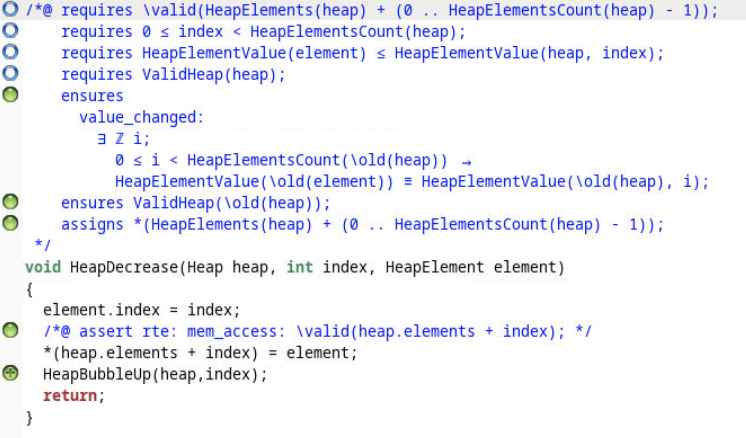
\includegraphics[width=10cm]{images/frama-c-HeapDecrease}
	\caption{Úspešné dokončení důkazu snížení hodnoty prvku haldy v prostředí Frama-C}
	\label{img:F-C-HeapDecrease}
\end{figure}


\subsection{Zvýšení hodnoty prvku}
\label{subsec:HeapIncrease}

Zvýšení hodnoty prvku haldy je operace nad haldou, která dokáže v čase $\mathcal{O}(1)$ změnit hodnotu vrcholu na daném indexu a následně v čase $\mathcal{O}(\log(n))$ opravit haldové uspořádání. Celková časová asymptotická složitost je tedy $\mathcal{O}(\log(n))$.

\begin{listing}[H]
	\caption{Kód a ACSL anotace zvýšení hodnoty prvku v hladě}
	\label{code:HeapIncrease}
	\begin{minted}{c}
/*@
  requires \valid(HeapElements(heap) + (0 .. HeapElementsCount(heap) - 1));
  requires 0 <= index < HeapElementsCount(heap);
  requires HeapElementValue(heap, index) <= HeapElementValue(element);
  requires ValidHeap(heap);

  assigns HeapElements(heap)[0 .. HeapElementsCount(heap) - 1];

  ensures value_changed:
    \exists integer i;
      0 <= i < HeapElementsCount(heap) ==>
        HeapElementValue(element) == HeapElementValue(heap, i);
  ensures ValidHeap(heap);
*/
void HeapIncrease(Heap heap, int index, HeapElement element) {
  element.index = index;
  heap.elements[index] = element;

  HeapBubbleDown(heap, index);
}
	\end{minted}
\end{listing}

Výpis kódu \ref{code:HeapIncrease} zobrazuje kód a ACSL anotaci funkce pro zvýšení hodnoty prvku v haldě. Jedna ze vstupních podmínek této funkce ověřuje, že hodnota, která nahrazuje původní hodnotu je doopravdy vyšší nebo stejná. Pokud by tato podmínka neplatila, volání algoritmu probublání dolů by neopravilo haldové uspořádání a nebylo by možné dokončit důkaz korektnosti algoritmu. Obrázek \ref{img:F-C-HeapIncrease} zobrazuje úspěšně dokončený důkaz korektnosti algoritmu zvýšení hodnoty prvku v haldě.

\begin{figure}[H]
	\centering
	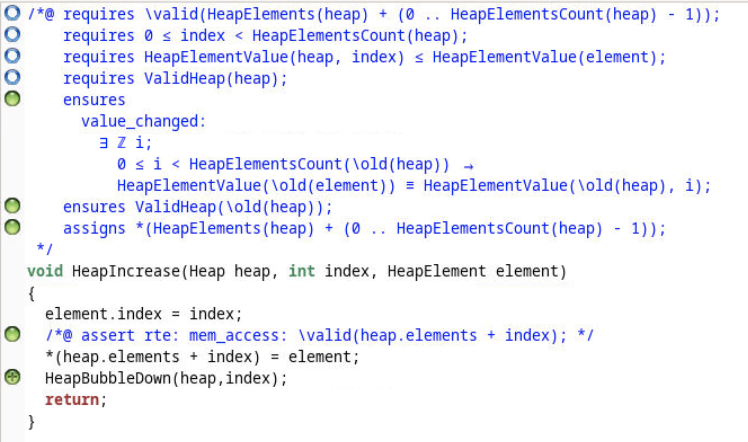
\includegraphics[width=10cm]{images/frama-c-HeapIncrease}
	\caption{Úspešné dokončení důkazu zvýšení hodnoty prvku haldy v prostředí Frama-C}
	\label{img:F-C-HeapIncrease}
\end{figure}


\section{Konstrukce haldy}
\label{subsec:HeapBuild}

Algoritmus konstrukce haldy je prvotní akce, která vytváří strukturu haldy a zajišťuje haldové uspořádání mezi prvky, ze kterých má být halda sestavena.

Implementace pomocí postupného vkládání jednotlivých prvků má časovou složitost $\mathcal{O}(n\log(n))$, jelikož musíme provést algoritmus vložení prvku, který má časovou složitost $\mathcal{O}(\log(n))$ pro každý prvek, ze kterého má být halda sestavena.

Tento algoritmus lze zefektivnit pomocí postupného opravování haldy probubláváním rodičovských vrcholů dolů. Algoritmus postupně zvětšuje podgraf spodního řezu haldou pomocí potomka až do té doby, než daný řez obsahuje všechny prvky, ze kterých měla být halda sestavena. Anotace algoritmus probublání dolů obsahují základní vstupní podmínky pro částečné opravení haldy, které tento postup splňují. Algoritmus sestavení haldy postupně nechává probublat dolů všechny rodičovské vrcholy od největšího index v poli až po kořen.

\begin{listing}[H]
	\caption{Kód a ACSL anotace zvýšení hodnoty prvku v hladě}
	\label{code:HeapBuild}
	\begin{minted}{c}
/*@
  requires 0 <= elementsCount <= elementsCapacity;
  requires \valid(elements + (0 .. elementsCount - 1));
  requires correctly_indexed:
    \forall integer i;
      0 <= i < elementsCount ==>
        HeapElementIndex(elements[i]) == i;

  assigns elements[0 .. elementsCount - 1];

  ensures count_same: HeapElementsCount(\result) == elementsCount;
  ensures capacity_same: HeapElementsCapacity(\result) == elementsCapacity;
  ensures ValidHeap(\result);
*/
Heap HeapBuild(HeapElement *elements, int elementsCount, int elementsCapacity) {
  Heap heap;
  heap.elements = elements;
  heap.elementsCount = elementsCount;
  heap.elementsCapacity = elementsCapacity;

  /*@
    loop invariant -1 <= index <= ((int)\floor(HeapElementsCount(heap) / 2)) - 1;

    loop invariant partially_valid_heap:
      \forall integer ancestor, descendant;
        index < ancestor < descendant < HeapElementsCount(heap)
        && IsParent(ancestor, descendant) ==>
          HasHeapProperty(heap, ancestor, descendant);

    loop assigns index, HeapElements(heap)[0 .. HeapElementsCount(heap) - 1];
    loop variant index;
  */
  for (int index = HeapInternalNodeCount(heap) - 1; index >= 0; index--) {
    HeapBubbleDown(heap, index);
  }

  return heap;
}
	\end{minted}
\end{listing}

Invarianty cyklu ve výpisu kód \ref{code:HeapBuild} zajišťují haldové uspořádání v spodním řezu haldou pomocí potomka s postupně snižujícím se indexem. Tento index bude po posledním kroku cyklu nastaven na hodnotu $-1$ a invariant spodního řezu haldou pomocí potomka tedy bude obsahovat celou haldu a bude zajišťovat haldové uspořádání v celé haldě.

%%---------------------------------------------------------------
%\chapter{Metody ladění při vývoji důkazu}
%%---------------------------------------------------------------
%
%\section{Zúžení vstupních podmínek}
%
%\section{Krokování}
%
%\section{Kontradikce}


%\section{Důkazy s referenčními datovými typy}
%
%V průběhu tvorby autor práce předával datovou strukturu mezi jednotlivými funkcemi pomocí odkazu na paměť. Princip předávání celé datové struktury pomocí odkazu umožňuje minimalizovat počet proměnných na zásobníku a všechny hodnoty ukládá v dynamické části paměti.
%
%Datová struktura reprezentující haldu se sestává z ukazatele na začátek pole, ve kterém jsou prvky haldy uložené, celočíselné hodnoty reprezentující aktuální počet uložených prvků v haldě a maximální kapacitu alokované paměti pole.
%
%Pokud je tato struktura předaná do některé obslužné funkce, která by s některými hodnotami pracovala, Frama-C a její WP plugin nemůže zajistit, že se v průběhu provádění dané funkce hodnoty nebudou měnit. Jelikož k hodnotám uloženým v haldě přistupujeme pomocí dereference ukazatele, může se teoreticky kdykoli stát, že hodnoty v paměti, kam daný ukazatel ukazuje již nejsou aktuální. Příkladem můžou být například vícevláknové aplikace.
%
%\section{Opravení haldy probubláním nahoru}
%
%Probublání prvku nahoru potřeba provést, pokud se v některý moment objeví v haldě prvek, který nesplňuje vlastnosti haldy a hodnota v daném vrcholu je menší, než hodnota v jeho rodiči. Tento stav nastává při vkládání prvku do haldy, kde se nový prvek přidá jako poslední prvek v téměř úplném binárním stromě a provede se probublání nahoru, aby se daný prvek dostal do správného místa v haldě tak, aby byla zajištěna vlastnost haldy pro všechny vrcholy rodičů a jejich synů.
%
%\subsection{Řez haldou}
%
%Pro důkaz autor využil řez haldou, který rozděluje graf haldy dle vlastnosti haldy (hodnota v rodiči je menší nebo rovna hodnotám v jeho synech) na dvě části. Korektní halda splňuje haldovu vlastnost mezi všemi dvojicemi rodič - syn. 
%Vrchní řez haldou tento predikát omezuje pouze na syny, kteří mají index v haldě ostře menší než problematický vrchol. Pro tyto vrcholy a jejich rodiče musí platit haldová vlastnost.
%Spodní řez haldou omezuje původní predikát na vrcholy, které mají index v haldě ostře větší než problematický index a pro ně také musí platit haldová vlastnost.
%Pro algoritmus probublání nahoru musí být zajištěno, že pouze problematický vrchol jakožto syn může porušovat haldoovu podmínku se svým rodičem.
%Princip důkazu spočívá v postupném posouvání vrchního a horního řezu do té doby, než horní řez není aplikován na žádný vrchol a spodní řez je aplikován na celou haldu. Tento moment nastává při pokusu o probublání kořene haldy. Jelikož žádný syn nemůže mít menší vrchol než kořen, predikát horního řezu je triviálně splněn. Dolní řež je poté speciálním případem původního predikátu korektní haldy. Tento princip je také zefektivněn v případě, že najdeme správné místo, kde by měl problematický vrchol zůstat, haldová vlastnost určitě platí pro vrcholy v horním i spodním řezu a nově i pro správně probublaný vrchol, což zaručuje plně splněný původní predikát korektní haldy.
%
%\section{Důkaz korektnosti algoritmu opravení haldy probubláním dolů}
%
%Podobně jako v případě probublání problémového prvku nahoru je u algoritmu probublání prvku haldy dolů využit řez haldou. Oproti řezu, který byl využit pro probublání nahoru tento řez mluví o rodičích. Protože v případě problémového prvku je možné, že pro oba jeho syny bude potrebušena haldová vlastnost. Kdežto pří probublání nahoru bylo přímo jasné mezi kterou dvojicí rodič syn je vlastnost porušená.

%---------------------------------------------------------------
\chapter{Hledání nejkratší cesty}
%---------------------------------------------------------------

\section{Dijkstrův algoritmus}

Dijkstrův algoritmu je grafový algoritmus pomocí kterého lze nalézt nejkratší cestu mezi dvěma vrcholy ohodnoceného orientovaného grafu. Algoritmus předpokládá nezáporné ohodnocení hran. Algoritmus hledá nejkratší cesty z vrcholu $s$ do všech vrcholů grafu. Algoritmus poté vypisuje pouze hrany z cílového vrcholu. Použitím binární minimové haldy je asymptotická časová složitost tohoto algoritmu $\mathcal{O}(|E|\log(|V|))$.

%---------------------------------------------------------------
\chapter{Vývojové prostředí}
%---------------------------------------------------------------

\section{Docker}

Docker a kotejnerové technologie umožňují spouštět kontejnery na společném jádře operačního systému. Liší se tímto od tradičních virtuálních strojů, které virtualizují jádro daného operačního systémů. Spuštěný kontejner se pomocí \cite{LinuxBible2020}

\subsection{Reverzní proxy}

\subsection{Editor kódu}

\subsection{Verifikační prostředí}

%---------------------------------------------------------------
\chapter*{Závěr}
\addcontentsline{toc}{chapter}{Závěr}
\markboth{Závěr}{Závěr}
%---------------------------------------------------------------

Tato práce se zaměřila na problematiku formálního důkazu implementace datové struktury binární minimové haldy. Podařilo se implementovat knihovnu v jazyce C s ACSL anotacemi, pomocí kterých byla dokázána korektnost jednotlivých knihovních funkcí.

Tato korektně implementovaná binární minimová halda byla použita v Dijkstrově algoritmu pro hledání nejkratší cesty v grafu. Rozšířením této práce by mohl být důkaz korektnosti tohoto algoritmu.

Součástí práce vzniklo také univerzální vývojové prostředí s možností editace kódu a spouštění formálního ověření bez nutnosti instalace těchto programů přímo v operačním systému. Toto vývojové prostředí lze také spustit na vzdáleném počítači (serveru) a editaci kódu a spouštění verifikace programů spouštět pomocí webového prohlížeče vzdáleně.